\documentclass[reqno,12pt]{amsart}

\usepackage[colorlinks=true]{hyperref}
\hypersetup{urlcolor=blue, citecolor=red}

\usepackage{amssymb,graphicx,color}
%\usepackage[english,francais]{babel}
\usepackage[latin1]{inputenc}

%\usepackage[cal=mathpi, frak=mma, scr=rsfs]{mathalfa}
%\usepackage[cal=mtc]{mathalfa}

%The Layout
\setlength{\oddsidemargin}{0pt}
\setlength{\evensidemargin}{0pt}
\setlength{\textheight}{42\baselineskip}
\setlength{\textwidth}{6in}
%\addtolength{\headheight}{0.7in}

\theoremstyle{plain}% default
\newtheorem{thm}{Theorem}[section]
\newtheorem{lem}{Lemma}[section]
\newtheorem{prop}{Proposition}[section]
\newtheorem{cor}{Corollary}[section]
\newtheorem{defs}{Definition}[section]
\newtheorem{prob}{Problem}[section]
\theoremstyle{definition}
\newtheorem{rmk}{Remark}[section]
\newtheorem{fact}{Fact}[section]

\newcommand{\NN}{{\mathbb{N}}}
\newcommand{\ZZ}{{\mathbb{Z}}}
\newcommand{\RR}{{\mathbb{R}}}
\newcommand{\CC}{{\mathbb{C}}}
\newcommand{\QQ}{{\mathbb{Q}}}
\newcommand{\bfu}{\mathbf{u}}
\newcommand{\bfv}{\mathbf{v}}
\newcommand{\bfw}{\mathbf{w}}
\newcommand{\bfe}{\mathbf{e}}
\newcommand{\bfa}{\mathbf{a}}
\newcommand{\bfb}{\mathbf{b}}
\newcommand{\bfg}{\mathbf{g}}
\newcommand{\bff}{\mathbf{f}}
\newcommand{\bfh}{\mathbf{h}}
\newcommand{\bfq}{\mathbf{q}}
\newcommand{\bfx}{\mathbf{x}}
\newcommand{\bfy}{\mathbf{y}}
\newcommand{\bfz}{\mathbf{z}}
\newcommand{\bfr}{\mathbf{r}}
\newcommand{\bfn}{\mathbf{n}}
\newcommand{\bfA}{\mathbf{A}}
\newcommand{\bfB}{\mathbf{B}}
\newcommand{\bfD}{\mathbf{D}}
\newcommand{\bfE}{\mathbf{E}}
\newcommand{\bfI}{\mathbf{I}}
\newcommand{\bfU}{\mathbf{U}}
\newcommand{\bfF}{\mathbf{F}}
\newcommand{\bfR}{\mathbf{R}}
\newcommand{\bfX}{\mathbf{X}}
\newcommand{\bfk}{\mathbf{k}}
\newcommand{\bfj}{\mathbf{j}}
\newcommand{\bfl}{\mathbf{l}}
\newcommand{\bfell}{\boldsymbol{\ell}}
\newcommand{\bfL}{\mathbf{L}}
\newcommand{\bfT}{\mathbf{T}}
\newcommand{\bfM}{\mathbf{M}}
\newcommand{\bfzero}{\mathbf{0}}
\newcommand{\fke}{\mathfrak{e}}
\newcommand{\fkE}{\mathfrak{E}}
\newcommand{\fkf}{\mathfrak{f}}
\newcommand{\fkF}{\mathfrak{F}}
\newcommand{\fkg}{\mathfrak{g}}
\newcommand{\fkG}{\mathfrak{G}}
\newcommand{\fkh}{\mathfrak{h}}
\newcommand{\fkH}{\mathfrak{H}}
\newcommand{\bfcurl}{\mbox{\bf curl}\;}
\newcommand{\bfalpha}{{\boldsymbol{\alpha}}}
\newcommand{\bfvarphi}{\boldsymbol{\varphi}}
\newcommand{\bfPhi}{\boldsymbol{\Phi}}
\newcommand{\bfpsi}{\boldsymbol{\psi}}
\newcommand{\bfxi}{\boldsymbol{\xi}}
\newcommand{\bfnabla}{\boldsymbol{\nabla}}
\newcommand{\bfdelta}{\boldsymbol{\delta}}
\newcommand{\bfomega}{\boldsymbol{\omega}}
\newcommand{\bfsigma}{\boldsymbol{\sigma}}
\newcommand{\bftau}{\boldsymbol{\tau}}
\newcommand{\bfeta}{\boldsymbol{\eta}}
\newcommand{\bfzeta}{\boldsymbol{\zeta}}
\newcommand{\bfkappa}{\boldsymbol{\kappa}}
\newcommand{\bfvarrho}{\boldsymbol{\varrho}}
\newcommand{\bfchi}{\boldsymbol{\chi}}
\newcommand{\define}{\stackrel{\mathrm{def}}{=}}
\newcommand{\Ccal}{{\mathcal C}}
\newcommand{\Acal}{{\mathcal A}}
\newcommand{\Bcal}{{\mathcal B}}
\newcommand{\Fcal}{{\mathcal F}}
\newcommand{\Scal}{{\mathcal S}}
\newcommand{\Ncal}{{\mathcal N}}
\newcommand{\Rcal}{{\mathcal R}}
\newcommand{\Qcal}{{\mathcal Q}}
\newcommand{\Gcal}{{\mathcal G}}
\newcommand{\Kcal}{{\mathcal K}}
\newcommand{\Xcal}{{\mathcal X}}
\newcommand{\Ycal}{{\mathcal Y}}
\newcommand{\Zcal}{{\mathcal Z}}
\newcommand{\Vcal}{{\mathcal V}}
\newcommand{\Wcal}{{\mathcal W}}
\newcommand{\per}{{\mathrm{per}}}
\newcommand{\ch}{{\mathrm{ch}}}
\newcommand{\loc}{{\mathrm{loc}}}
\newcommand{\zave}[1]{\dot{#1}}
\newcommand{\Ecal}{{\mathcal E}}
\newcommand{\Mcal}{{\mathcal M}}
\newcommand{\Pcal}{{\mathcal P}}
\newcommand{\Dcal}{{\mathcal D}}
\newcommand{\Tcal}{{\mathcal T}}
\newcommand{\Ucal}{{\mathcal U}}
\newcommand{\Lcal}{{\mathcal L}}
\newcommand{\Ocal}{{\mathcal O}}
\newcommand{\Gr}{\mathrm{G}}
\newcommand{\Rey}{\mathrm{Re}}
\newcommand{\rmD}{\mathrm{D}}
\newcommand{\rmH}{\mathrm{H}}
\newcommand{\rmP}{\mathrm{P}}
\newcommand{\rmS}{\mathrm{S}}
\newcommand{\rmKo}{\mathrm{Ko}}
\newcommand{\rmKr}{\mathrm{Kr}}
\newcommand{\rmd}{\mathrm{d}}
\newcommand{\rmw}{\mathrm{w}}
\newcommand{\rmv}{\mathrm{v}}
\newcommand{\rmreg}{\mathrm{reg}}
\newcommand{\rmb}{\mathrm{b}}
\newcommand{\rmg}{\mathrm{g}}
\newcommand{\rmc}{\mathrm{c}}
\newcommand{\rmr}{\mathrm{r}}
\newcommand{\rms}{\mathrm{s}}
\newcommand{\sfA}{\mathsf{A}}
\newcommand{\sfD}{\mathsf{D}}
\newcommand{\sfT}{\mathsf{T}}
\newcommand{\sfI}{\mathsf{I}}
\newcommand{\sfJ}{\mathsf{J}}
\newcommand{\sfS}{\mathsf{S}}
\newcommand{\sfsigma}{\mathsf{\sigma}}
\newcommand{\sftau}{\mathsf{\tau}}
\newcommand{\sgn}{\operatorname{sgn}}
\newcommand{\Id}{\operatorname{Id}}
\newcommand{\tr}{{\operatorname{tr}}}
\newcommand{\supp}{\operatorname*{supp}}
\newcommand{\Tr}{\operatorname{Tr}}
\newcommand{\Cyl}{\operatorname{\mathcal{C}_{yl}}}
\newcommand{\Syl}{\operatorname{\mathcal{S}_{yl}}}
\newcommand{\nse}{{\operatorname{nse}}}
\newcommand{\cyl}{{\operatorname{cyl}}}
\newcommand{\sss}{{\operatorname{sss}}}
\newcommand{\fpsss}{{\operatorname{fpsss}}}
\newcommand{\wsss}{{\operatorname{wsss}}}
\newcommand{\tasss}{{\operatorname{tasss}}}
\newcommand{\inv}{{\operatorname{inv}}}
\newcommand{\Linv}{{\operatorname{L-inv}}}
\newcommand{\Einv}{{\operatorname{E-inv}}}
\newcommand{\sinv}{{\operatorname{\sigma-inv}}}
\newcommand{\Piinv}{{\operatorname{\Pi-inv}}}
\newcommand{\average}[1]{\langle{#1}\rangle}
\newcommand{\dual}[1]{\langle{#1}\rangle}
\newcommand{\inner}[1]{({#1})}
\newcommand{\dinner}[1]{(\!({#1})\!)}
\newcommand{\Lim}{\operatorname*{\textsc{Lim}}_{T\rightarrow \infty}}
\newcommand{\co}{\operatorname*{\text{co}}}
\newcommand{\paratitle}[1]{\vspace{\baselineskip} \noindent \emph{{#1}}}
%\newcommand{\comment}[1]{\textcolor{red}{\framebox{\parbox{0.9\textwidth}{\textbf{#1}}}}}
\newcommand{\comment}[1]{\textcolor{red}{\textbf{#1}}}
\newcommand{\doshow}[1]{#1}
\newcommand{\dontshow}[1]{}
\newcommand{\extra}[1]{\dontshow{#1}} % use \show to show the extra stuff or \donotshow not to show it

%\mathchardef\mhyphen="2D

\renewcommand{\subjclassname}{$2020$ Mathematics Subject Classification}

\renewcommand{\theenumi}{\roman{enumi}}

\begin{document}
\numberwithin{equation}{section}

% Article info

\title[Euler-Maruyama strong order 1 for Random ODEs]{The Euler-Maruyama scheme for random ordinary differential equations is of strong order 1}

\author[R. Rosa]{Ricardo M. S. Rosa}

%\author[R. Temam]{Roger M. Temam}

\address[Ricardo M. S. Rosa]{Instituto de Matem\'atica, Universidade Federal do Rio de Janeiro, Brazil}
%\address[Roger M. Temam]{Indiana University, Bloomington, IN, USA}

\email[R. Rosa]{rrosa@im.ufrj.br}
%\email[R. Temam]{temam@indiana.edu}

\date{\today}

%\thanks{This work was partly supported by the CNPq, Bras\'{\i}lia, Brazil and by the NSF grant ???.}

\subjclass[2020]{76D05, 76D06, 35Q30, 37L99}
\keywords{random ordinary differential equations, Euler-Maruyama method, strong convergence, It\^o process}.

\begin{abstract}
It is well known that the Euler-Maruyama method of approximating a random ordinary differential equation $\mathrm{d}X_t/\mathrm{d}t = f(t, X_t, Y_t)$ driven by a stochastic process $\{Y_t\}_t$ with $\theta$-H\"older sample paths is estimated to be of strong order $\theta$ with respect to the time step, provided e.g. $f=f(t, x, w)$ is globally Lipschitz. Here, we show that, if $\{Y_t\}_t$ is an It\^o process with bounded drift and diffusion and $f$ is twice continuously differentiable and is bounded along with its derivatives, then the Euler-Maruyama method is actually of strong order 1. The estimate follows from not estimating part of the local error and, instead, adding up the local steps and estimating the compound error via the It\^o formula and the It\^o isometry. We complement the result by giving examples where some of the conditions are not met and the order of convergence seems indeed to be less than 1.
\end{abstract}

\maketitle

\section{Introduction}

Here, we consider the following initial value problem for a \textbf{random ordinary differential equation (RODE)}:
\begin{equation}
  \label{rodeeq}
  \begin{cases}
    \displaystyle \frac{\mathrm{d}X_t}{\mathrm{d} t} = f(t, X_t, Y_t), \qquad t \geq 0, \\
    \left. X_t \right|_{t = 0} = X_0,
  \end{cases}
\end{equation}
where $\{Y_t\}$ is a (real) stochastic process with continuous sample paths, $f:[0, \infty) \times \mathbb{R} \times\mathbb{R} \rightarrow \mathbb{R}$ is continuous, and $X_0$ is a real random variable on a sample space $\Omega$.

The Euler-Maruyama method for solving this initial value problem in a time interval $[0, T]$ consists in considering a uniform time mesh $t_j = j\Delta t$, $j = 0, \ldots, N$, with fixed time step $\Delta t = T/N$, for a given $N\in \mathbb{N}$. Then, the Euler-Maruyama scheme takes the form
\begin{equation}
  \label{emscheme}
  X_{t_j}^N = X_{t_{j-1}}^N + \Delta t f(t_{j-1}, X_{t_{j-1}}^N, Y_{t_{j-1}}), \qquad j = 1, \ldots, N,
\end{equation}
with the initial condition
\begin{equation}
  \label{iccondition}
  X_0^N = X_0.
\end{equation}

One of our interests is to drive the equation with an \textbf{It\^o process} $\{Y_t\}_{t\geq 0}$, satisfying
\begin{equation}
  \label{itoprocess}
  \mathrm{d}Y_t = A_t \;\mathrm{d}t + B_t \;\mathrm{d}W_t,
\end{equation}
where $\{W_t\}_{t\geq 0}$ is a Wiener process and $\{A_t\}_{t \geq 0}$ and $\{B_t\}_{t \geq 0}$ are stochastic processes adapted to the $\{W_t\}_{t\geq 0}$.

In the case that $f=f(t, x, y)$ is twice continuously differentiable, the It\^o formula is applicable and yields
\begin{multline}
  \label{itoformula}
  \mathrm{d}f(t, x, Y_t) = \left(\partial_t f(t, x, Y_t) + A_t \partial_y f(t, x, Y_t)  + \frac{B_t^2}{2}\partial_{yy}f(t, x, Y_t) \right) \;\mathrm{d}t \\ + B_t \partial_y f(t, x, Y_t)\;\mathrm{d}W_t,
\end{multline}
for every fixed $x\in \mathbb{R}$.

We show that, if $\{A_t\}_t$, $\{B_t\}_t$ are uniformly bounded on $[0, T]$ (uniformly for all sample paths) and $f$, $\partial_t f$, $\partial_x f$, $\partial_y f$, and $\partial_{yy}f$ are uniformly bounded on $[0, T]\times \mathbb{R}\times \mathbb{R}$, then the Euler-Maruyama method is of strong order 1, i.e. there exists $C>0$ such that
\begin{equation}
  \mathbb{E}\left[ \left| X_{t_j} - X_{t_j}^N \right| \right] \leq C \Delta t, \qquad \forall N \in \mathbb{N},  \Delta t = \frac{T}{N},
\end{equation}
where $\mathbb{E}[\cdot]$ indicates the expectation of a random variable on $\Omega$ (see Theorem \ref{EMstrongorder1}).

We summarize here the main tricks we use to accomplish such error estimate:
\begin{enumerate}
  \item We assume the noise is an It\^o process, so we can use the It\^o isometry at some point;
  \item We use the It\^o formula to separate the most problematic/rough part of the noise;
  \item We do not estimate this problematic term locally at each time step;
  \item Instead, we add up the difference equation for the time steps and write the error in terms of a time integral of this rough part of the noise;
  \item We then use the It\^o isometry to estimate this integral term by $\Delta t$;
  \item We use a variation of the discrete Gronwall Lemma to estimate the added up inequality.
\end{enumerate}

In order to make the main idea clear cut, here are the options we have for estimating the rough part of the noise:
\begin{enumerate}
  \item If the local error $e_j$ of the rough part of the noise, at the $j$th time step, is bounded as
    $$
    \mathbb{E}[|e_j|] \lesssim \Delta t^{3/2},
    $$
    as usual, then adding them up leads to 
    $$
      \sum \mathbb{E}[|e_j|] \lesssim N\Delta t^{3/2} = T\Delta t^{1/2}.
    $$
    \item If we use the It\^o isometry locally, we still get the local error as
    $$
      \mathbb{E}[|e_j|] \leq \mathbb{E}[|e_j|^2]^{1/2} \lesssim \left(\Delta t^3 \right)^{1/2} = \Delta t^{3/2},
    $$
    and adding that up still leads to an error of order $\Delta t^{1/2}$.
    \item If, instead, we first add the terms up, then $\sum e_j$ becomes an integral over $[0, T]$ with respect to the Wiener noise, so that we can use the It\^o isometry on the added up term and obtain
    \begin{multline*}
      \mathbb{E}\left[ \left| \sum e_j \right| \right] \lesssim \left(\mathbb{E}\left[ \left| \sum e_j \right|^2 \right]\right)^{1/2} = \left( \sum \mathbb{E}[|e_j|^2] \right)^{1/2} \\
      = \left( \sum \Delta t^3 \right)^{1/2} = \left( \Delta t^2 \right)^{1/2} = \Delta t.
    \end{multline*}
    and we finally get the error to be of order 1.
\end{enumerate}

\section{Strong order of convergence}

We assume $f=f(t, x, y)$ is twice continuously differentiable with
\begin{align}
  \label{Mfassumption} M_f & = \sup_{t, x, y} |f(t, x, y)| < \infty, \\
  \label{Ltassumption} L_t & = \sup_{t, x, y} |\partial_t f(t, x, y)| < \infty \\
  \label{Lxassumption} L_x & = \sup_{t, x, y} |\partial_x f(t, x, y)| < \infty \\
  \label{Lyassumption} L_y & = \sup_{t, x, y} |\partial_y f(t, x, y)| < \infty \\
  \label{Lyyassumption} L_{yy} & = \sup_{t, x, y} |\partial_y^2 f(t, x, y)| < \infty,
\end{align}
where the suprema are taken for $(t, x, y) \in [0, T] \times \mathbb{R} \times \mathbb{R}$.

We also assume the drift and diffusion of the It\^o process $\{Y_t\}_t$ are uniformly bounded,
\begin{align}
  \label{MAassumption} M_A & = \sup_\omega \sup_{t, x, y} |A_t(\omega)| < \infty, \\
  \label{MBassumption} M_B & = \sup_\omega\sup_{t, x, y} |B_t(\omega)| < \infty,
\end{align}
where the suprema are taken for $t\in [0, T]$ and for samples in all sample space $\omega\in \Omega$.

\subsection{A single step}

Here we obtain an expression for a time step, from $t$ to $t + \Delta t$, which will be suitable for a proper estimate later on.

The exact solution satisfies, for any $\tau \geq 0$, and, in particular, for $0\leq \tau \leq \Delta t$, 
$$
X_{t + \tau} = X_t + \int_t^{t + \tau} f(s, X_s, Y_s) \;\mathrm{d}s.
$$
The Euler-Maruyama step is given by
$$
X_{t+\Delta t}^n = X_t^n + \Delta t f(t, X_t^n, Y_t).
$$
If we consider a linear interpolation, we can also write
$$
X_{t + \tau}^n = X_t^n + \tau f(t, X_t^n, Y_t),
$$
for $0\leq \tau \leq \Delta t$.

Subtracting, we obtain
$$
X_{t + \tau} - X_{t + \tau}^n = X_t - X_t^n + \int_t^{t + \tau} \left( f(s, X_s, Y_s) - f(t, X_t^n, Y_t) \right)\;\mathrm{d}s.
$$

We arrange the integrand as
\begin{align*}
f(s, X_s, Y_s) - f(t, X_t^n, Y_t) = & f(s, X_s, Y_s) - f(s, X_t, Y_s) \\ 
 & + f(s, X_t, Y_s) - f(s, X_t^n, Y_s) \\
 & + f(s, X_t^n, Y_s) - f(t, X_t^n, Y_t).
\end{align*}

This yields
\begin{align*}
X_{t + \tau} - X_{t + \tau}^n  = & X_t - X_t^n \\
= &  \int_t^{t + \tau} \left( f(s, X_s, Y_s) - f(s, X_t, Y_s) \right)\;\mathrm{d}s \\ 
 & + \int_t^{t + \tau} \left( f(s, X_t, Y_s) - f(s, X_t^n, Y_s) \right)\;\mathrm{d}s \\
 & + \int_t^{t + \tau} \left( f(s, X_t^n, Y_s) - f(t, X_t^n, Y_t) \right)\;\mathrm{d}s.
\end{align*}

For the integral of the last pair of terms, we use the It\^o formula on $Z_s = f(s, X_t^n, Y_s)$ and write
\begin{align*}
\int_t^{t + \tau} & \left(f(s, X_t^n, Y_s) - f(t, X_t^n, Y_t) \right)\;\mathrm{d}s  = \int_t^{t + \tau} \int_t^s \mathrm{d}Z_\xi \;\mathrm{d}s \\
& = \int_t^{t + \tau} \int_t^s \left(\partial_\xi f(\xi, X_t^n, Y_\xi) + A_\xi \partial_y f(\xi, X_t^n, Y_\xi)  + \frac{B_\xi^2}{2}\partial_{yy}f(\xi, X_t^n, Y_\xi) \right) \;\mathrm{d}s\;\mathrm{d}t \\ 
& \quad + \int_t^{t + \tau} \int_t^s B_\xi \partial_y f(\xi, X_t^n, Y_\xi)\;\mathrm{d}W_\xi\;\mathrm{d}s.
\end{align*}
Using Fubini's Theorem, the last integral is rewritten as
\begin{multline}
\label{fubini}
\int_t^{t + \tau} \int_t^s B_\xi \partial_y f(\xi, X_t^n, Y_\xi)\;\mathrm{d}W_\xi\;\mathrm{d}s 
  = \int_t^{t + \tau} \int_\xi^{t + \tau} B_\xi \partial_y f(\xi, X_t^n, Y_\xi) \;\mathrm{d}s \;\mathrm{d}W_\xi \\
  = \int_t^{t+\tau} (t + \tau - \xi) B_\xi \partial_y f(\xi, X_t^n, Y_\xi) \;\mathrm{d}W_\xi.
\end{multline}

We rearrange these terms and write, for $\tau = \Delta t$ and $t = t_{j-1} = (j-1)\Delta t$,
\begin{equation}
\label{stepexpression}
X_{t_j} - X_{t_j}^n  = X_{t_{j-1}} - X_{t_{j-1}}^n  + I_{j-1}^{1} + I_{j-1}^{2} + I_{j-1}^{3},
\end{equation}
where
$$
I_j^{1} = \int_{t_j}^{t_{j+1}} \left( f(s, X_{t_j}, Y_s) - f(s, X_{t_j}^n, Y_s) \right)\;\mathrm{d}s,
$$
\begin{multline*}
  I_j^2 =  \int_{t_j}^{t_{j+1}}  \left( f(s, X_s, Y_s) - f(s, X_{t_j}, Y_s) \right)\;\mathrm{d}s \\ 
 +  \int_{t_j}^{t_{j+1}} \int_{t_j}^s \left(\partial_\xi f(\xi, X_{t_j}^n, Y_\xi) + A_\xi \partial_y f(\xi, X_{t_j}^n, Y_\xi)  + \frac{B_\xi^2}{2}\partial_{yy}f(\xi, X_{t_j}^n, Y_\xi) \right) \;\mathrm{d}t,
\end{multline*}
and
$$
I_j^3 = \int_{t_j}^{t_{j+1}}  (t_{j+1} - \xi) B_\xi \partial_y f(\xi, X_{t_j}^n, Y_\xi) \;\mathrm{d}W_\xi.
$$

\subsection{Local estimates}

The term $I_j^1$ is estimated using that $f=f(t, x, y)$ is globally Lipschitz in $x$, so that
$$
\left| f(s, X_t, Y_s) - f(s, X_t^n, Y_s) \right| \leq L_x |X_t - X_t^n|.
$$
Hence,
\begin{multline*}
\left|  \int_{t_j}^{t_{j+1}} \left( f(s, X_{t_j}, Y_s) - f(s, X_{t_j}^n, Y_s)  \right) \;\mathrm{d}s \right| \leq   \int_{t_j}^{t_{j+1}} \left| f(s, X_{t_j}, Y_s) - f(s, X_{t_j}^n, Y_s)  \right| \;\mathrm{d} s \\ \leq L_x |X_{t_j} - X_{t_j}^n| \Delta t.
\end{multline*}
This means
\begin{equation}
\label{I1estimate}
\left| I_j^1 \right| \leq L_x |X_{t_j} - X_{t_j}^n| \Delta t.
\end{equation}

For $I_j^2$, the first term is estimated as
$$
\left| f(s, X_s, Y_s) - f(s, X_t, Y_s) \right| \leq L_x |X_s - X_t| \leq L_x \int_t^s |f(\sigma, X_\sigma, Y_\sigma)| \;\mathrm{d}\sigma \leq L_x M_f (s - t).
$$
This yields, upon integration,
\begin{multline*}
\left|  \int_{t_j}^{t_{j+1}} \left(f(s, X_s, Y_s) - f(s, X_{t_j}, Y_s) \right) \;\mathrm{d}s \right| \leq  \int_{t_j}^{t_{j+1}} \left| f(s, X_s, Y_s) - f(s, X_{t_j}, Y_s) \right| \;\mathrm{d} s \\
\leq \frac{L_x M_f}{2} \Delta t^2.
\end{multline*}

The double integral is estimated as
\begin{multline}
   \left|  \int_{t_j}^{t_{j+1}}  \int_\xi^{t_{j+1}} \left(\partial_\xi f(\xi, X_{t_j}^n, Y_\xi) + A_\xi \partial_y f(\xi, X_{t_j}^n, Y_\xi)  + \frac{B_\xi^2}{2}\partial_{yy}f(\xi, X_{t_j}^n, Y_\xi) \right) \;\mathrm{d}t \right| \\
   \leq \int_{t_j}^{t_{j+1}}  \int_\xi^{t_{j+1}} \left(L_t + M_A L_y  + \frac{M_B^2}{2}L_{yy} \right) \;\mathrm{d}t \\
   = \frac{1}{2}\tau^2\left(L_t + M_A L_y  + \frac{M_B^2}{2}L_{yy} \right).
\end{multline}
Hence,
\begin{equation}
\label{I2estimate}
\left| I_j^2 \right| \leq M\Delta t^2,
\end{equation}
where
$$
M = \frac{1}{2}\left(L_x M_f + L_t + M_A L_y  + \frac{M_B^2}{2}L_{yy} \right).
$$

\begin{rmk}\tiny
Notice that, at this point, we did not estimate the last integral, otherwise we are not able to obtain the strong order 1 estimate, only 1/2. Indeed, if we use Fubini and the It\^o isometry in the last integral, we find
\begin{align*}
  \mathbb{E} & \left[ \left( \int_t^{t + \tau} \int_t^s B_\xi \partial_y f(\xi, X_t^n, Y_\xi)\;\mathrm{d}W_\xi\;\mathrm{d}s \right)^2\right] = \mathbb{E} \left[ \left( \int_t^{t + \tau} \int_\xi^{t+\tau} B_\xi \partial_y f(\xi, X_t^n, Y_\xi) \;\mathrm{d}s\;\mathrm{d}W_\xi \right)^2\right] \\
  & = \int_t^{t + \tau} \mathbb{E} \left[ \left( \int_\xi^{t+\tau} B_\xi \partial_y f(\xi, X_t^n, Y_\xi) \;\mathrm{d}s \right)^2\right] \;\mathrm{d}\xi  \leq  \int_t^{t + \tau}  \left( \int_\xi^{t+\tau} M_B^2 L_y \;\mathrm{d}s \right)^2\;\mathrm{d}\xi \\
  & \leq  \int_t^{t + \tau}  M_B^2 L_y (t + \tau - \xi)^2\;\mathrm{d}\xi  = \left. - \frac{1}{3} M_B^2 L_y^2 (t + \tau - \xi)^3 \right]_t^{t+\tau}  = \frac{1}{3} M_B^2 L_y^2 \tau^3,
\end{align*}
so that
\begin{equation}
\sqrt{\mathbb{E} \left[ \left( \int_t^{t + \tau} \int_t^s B_\xi \partial_y f(\xi, X_t^n, Y_\xi)\;\mathrm{d}W_\xi\;\mathrm{d}s \right)^2\right]} \leq \frac{\sqrt{3}}{3} M_B L_y \tau^{3/2}.
\end{equation}
After adding up $n$ times, we end up with a $\tau^{1/2}$ estimate, which is not sufficient.
\end{rmk}

\subsection{Integral estimate}

The third term $I_j^3$ is not estimated for each $j$ separately. Instead, we estimate its summation over $j$. Notice
\begin{multline*}
\sum_{i=0}^{j-1} I_i^3 = \sum_{i=0}^{j-1} \int_{t_i}^{t_{i+1}} (t_{i+1} - \xi) B_\xi \partial_y f(\xi, X_{t_i}^n, Y_\xi)  \;\mathrm{d}W_\xi \\
 = \int_0^{t_j} \left([\xi/\Delta t + 1]\Delta t - \xi\right) B_\xi \partial_y f(\xi, X_{[\xi/\Delta t]\Delta t}^n, Y_\xi) \;\mathrm{d}W_\xi,
\end{multline*}
where $[r]$ denotes the largest integer below a real number $r$.

For this term, we estimate its strong norm, i.e. first moment. This is estimated using the Lyapunov inequality, the It\^o formula and the It\^o isometry, as follows
\begin{align*}
  \mathbb{E}&\left[ \left| \int_0^{t_j} \left([\xi/\Delta t + 1]\Delta t - \xi\right) B_\xi \partial_y f(\xi, X_{[\xi/\Delta t]\Delta t}^n, Y_\xi) \;\mathrm{d}W_\xi\right| \right] \\
   & \leq \mathbb{E}\left[ \left( \int_0^{t_j} \left([\xi/\Delta t + 1]\Delta t - \xi\right) B_\xi \partial_y f(\xi, X_{[\xi/\Delta t]\Delta t}^n, Y_\xi)\;\mathrm{d}W_\xi \right)^2 \right]^{1/2} \\
   & =  \left(\int_0^{t_j} \mathbb{E}\left[ \left(\left([\xi/\Delta t + 1]\Delta t - \xi\right) B_\xi \partial_y f(\xi, X_{[\xi/\Delta t]\Delta t}^n, Y_\xi)\right)^2 \right]\;\mathrm{d}\xi \right)^{1/2}\\
   & \leq \left(\int_0^{t_j} \left(\left([\xi/\Delta t + 1]\Delta t - \xi\right)^2\mathbb{E}\left[ \left( B_\xi \partial_y f(\xi, X_{[\xi/\Delta t]\Delta t}^n, Y_\xi)\right)^2 \right]\right) \;\mathrm{d}\xi \right)^{1/2}\\
   & \leq \left(\int_0^{t_j} \Delta t^2 M_B^2 L_y^2 \;\mathrm{d}\xi \right)^{1/2}.
\end{align*}

Thus,
\begin{equation}
  \label{I3estimate}
  \mathbb{E}\left[ \left| \sum_{i=0}^{j-1} I_j^3 \right| \right] \leq M_B L_y t_j^{1/2} \Delta t.
\end{equation}

\subsection{Iterating the steps}

Iterating \eqref{stepexpression} and assuming that $X_0^n = X_0$, we find
\begin{equation}
  \label{iteratedexpression}
  X_{t_j} - X_{t_j}^n = \sum_{i=0}^{j-1} I_j^1 + \sum_{i=0}^{j-1} I_j^2 + \sum_{i=0}^{j-1} I_j^3.
\end{equation}

We estimate the first moment as
\begin{equation}
 \mathbb{E}\left[| X_{t_j} - X_{t_j}^n |\right] \leq \sum_{i=0}^{j-1} \mathbb{E}\left[| I_j^1|\right] + \sum_{i=0}^{j-1} \mathbb{E}\left[|I_j^2 |\right] + \mathbb{E}\left[ \left| \sum_{i=0}^{j-1} I_j^3 \right| \right].
\end{equation}
Using \eqref{I1estimate}, \eqref{I2estimate}, and \eqref{I3estimate}, we obtain
\begin{multline}
\label{iteratedestimate}
 \mathbb{E}\left[| X_{t_j} - X_{t_j}^n |\right] \leq L_x \sum_{i=0}^{j-1} \mathbb{E}\left[|X_{t_j} - X_{t_j}^n|\right]\Delta t + \sum_{i=0}^{j-1} C\Delta t^2 + M_B L_y t_j \Delta t \\
 \leq L_x \sum_{i=0}^{j-1} \mathbb{E}\left[|X_{t_i} - X_{t_i}^n|\right]\Delta t + C_T \Delta t,
\end{multline}
where
$$
C_T = M + M_B L_yT^{1/2}.
$$

Now, we show by induction that
$$
 \mathbb{E}\left[| X_{t_j} - X_{t_j}^n |\right] \leq C_T e^{L_x t_j}\Delta t .
$$
This is trivially true for $j=0$. Now suppose it is true up to $j-1$. It follows from \eqref{iteratedestimate} that
$$
 \mathbb{E}\left[| X_{t_j} - X_{t_j}^n |\right] \leq L_x \sum_{i=0}^{j-1} C_T \Delta t e^{L_x t_i}\Delta t + C_T \Delta t = C_T \Delta t\left( 1 + L_x \Delta t \sum_{i=0}^{j-1}  e^{L_x t_i} \right).
$$
Using that $1 + r \leq e^r$, with $r=L_x\Delta t$ and $t_i + \Delta t = t_{i+1}$, we see that
$$
L_x \Delta t \leq e^{L_x \Delta t} - 1,
$$
which telescopes the sum and yields
$$
 \mathbb{E}\left[| X_{t_j} - X_{t_j}^n |\right] \leq C_T \Delta t\left( 1 + (e^{L_x \Delta t} - 1)\sum_{i=0}^{j-1}  e^{L_x t_i} \right) = C_T \Delta t  \left(1 + (e^{L_x j\Delta t} - 1) \right).
$$
Hence,
$$
 \mathbb{E}\left[| X_{t_j} - X_{t_j}^n |\right] \leq C_T e^{L_x t_j}\Delta t ,
$$
which completes the induction. Hence, we have proved the following result.

\begin{thm}
  \label{EMstrongorder1}
  Consider the initial value problem \eqref{rodeeq}, on a time interval $[0, T]$, with $T > 0$, and assume the noise is given by \eqref{itoprocess}, with \eqref{MAassumption} and \eqref{MBassumption}. Suppose $f=f(t, x, y)$ is twice continuously differentiable, with \eqref{Mfassumption}-\eqref{Lyyassumption}. Let $\{X_t\}_{t\geq 0}$ be the solution of \eqref{rodeeq}. Let $N\in \mathbb{N}$ and let $\{X_{t_j}^N\}_{j=0, \ldots, N}$ be the solution of the Euler-Maruyama method \eqref{emscheme}-\eqref{iccondition}. Then,
  \begin{equation}
  \mathbb{E}\left[ \left| X_{t_j} - X_{t_j}^N \right| \right] \leq C_T e^{L_x t_j} \Delta t, \qquad j = 0, \ldots, N, \;\forall N \in \mathbb{N},  \Delta t = \frac{T}{N},
\end{equation}
  where
  \begin{equation}
    C_T = \frac{1}{2}\left(L_x M_f + L_t + M_A L_y  + \frac{M_B^2}{2}L_{yy} \right) + M_B L_yT^{1/2}.
  \end{equation}
\end{thm}

We end this section by abstracting away the Gronwall type inequality we use \textcolor{red}{(this is probably written somewhere, and I need to find the source)}:
\begin{lem}
Let $(e_j)_j$ be a (finite or infinite) sequence of positive numbers satisfying
\begin{equation}
  \label{integralgronwall}
  e_j \leq a \sum_{i=0}^{j-1} e_i + b,
\end{equation}
with $e_0 = 0$, where $a, b > 0$. Then,
\begin{equation}
  \label{estimateintegralgronwall}
  e_j \leq b e^{aj}, \qquad \forall j.
\end{equation}
\end{lem}

\begin{proof}
  The result is trivially true for $j=0$. Suppose, by induction, that the result is true up to $j-1$. Then,
  $$
  e_j \leq a \sum_{i=0}^{j-1} be^{ai} + b = b \left(a \sum_{i=0}^{j-1} e^{ai} + 1\right).
  $$
  Using that $1 + a \leq e^a$, we have $a \leq e^a - 1$, hence
  $$
  e_j \leq b\left((e^a - 1)\sum_{i=0}^{j-1} e^{ia} + 1\right).
  $$
  Using that $\sum_{i=0}^{j-1} \theta^i = (\theta^j - 1)(\theta - 1)$, with $\theta = e^a$, we see that
  $$
  (e^a - 1)\sum_{i=0}^{j-1} e^{ia} \leq e^{ja} - 1,
  $$
  so that
  $$
  e_j \leq be^{ja},
  $$
  which completes the induction.
\end{proof}

\section{Numerical examples}

\subsection{Lower-order converge}

\begin{figure}
  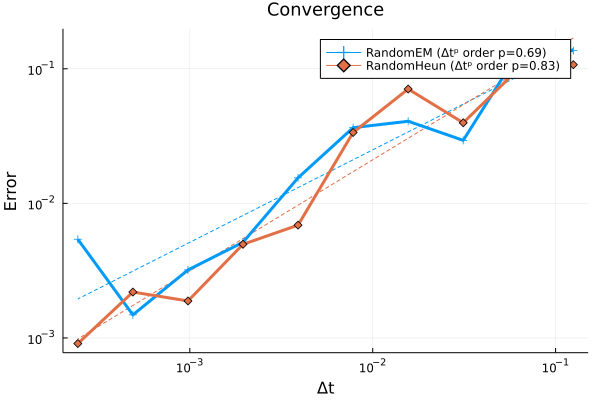
\includegraphics{img/plot_13.png}
\end{figure}

For a lower order convergence, below order $1$, we take the noise $\{Y_t\}_t$ to be the transport process defined by
$$
Y_t = \sin(t/Z)^{1/3},
$$
where $Z$ is a beta random variable $Z \sim B(\alpha, \beta)$. Notice $Z$ takes values strictly within $(0, 1)$ and, hence, $\sin(t/Z)$ can have arbitrarily high frequencies and, hence, go through the critic value $y = 0$ extremely often.

\textcolor{red}{(Need to remove the Heun method and do more tests)}.

\section*{Acknowledgments}


\begin{thebibliography}{25}


\end{thebibliography}

\end{document}